\section{Tecnologías y herramientas utilizadas}
Como se mencionó anteriormente, se tomo la decisión de implementar la herramienta como una
aplicación web. En esta sección presentaremos las herramientas y tecnologías empleadas para el
desarrollo del sistema con un enfoque web (\figref{fig:stack-tecnologias}).

\begin{figure}[!htpb]
\centering
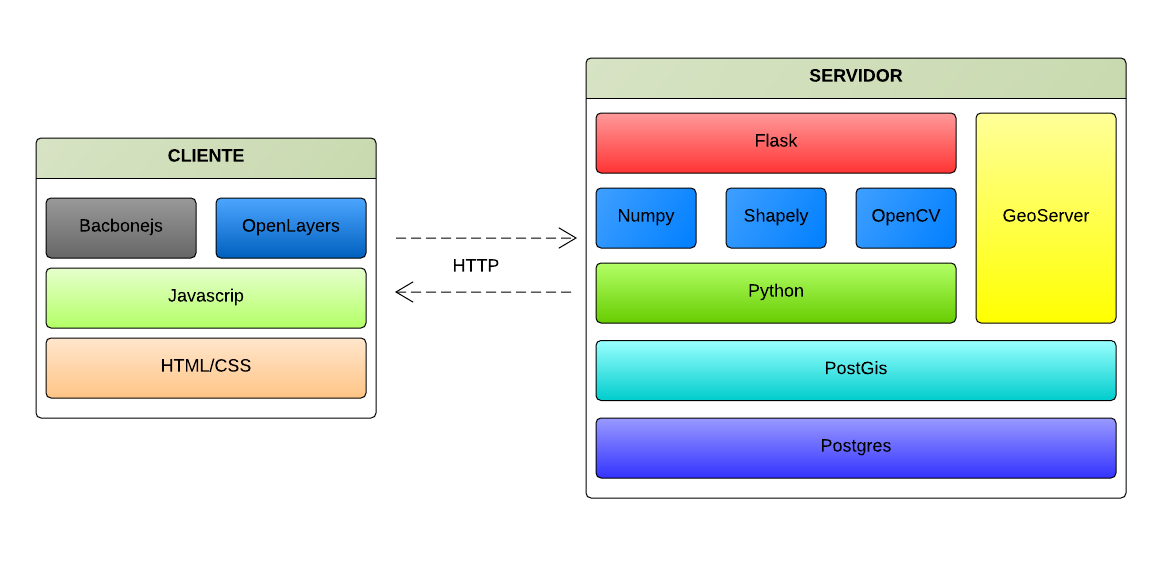
\includegraphics[width=1\textwidth]{capitulo-5/graphics/stack-tecnologias.png}
\caption{\label{fig:stack-tecnologias}Pila de tecnologías utilizadas para el desarrollo.}
\end{figure}

La capa de presentación fue desarrollada puramente en javascript, html y css, con el framework
Backbonejs \footnote{http://backbonejs.org/} donde la comunicación con la capa de servicios se
encuentra dada por peticiones Ajax. Para la visualización e interacción como mapas se utilizó
OpenLayers \footnote{http://openlayers.org/}. Como servidor web para la publicación de la capa de
presentación se utilizó Apache\footnote{https://httpd.apache.org/} en su versión 2, aunque se
podría utilizarse cualquier otro servidor web HTTP.

La capa de negocios, se encuentra desarrollada en Python, en donde para la capa de servicios se
utilizó Flask\footnote{http://flask.pocoo.org/} un framework minimalista para Python. Para llevar
a cabo análisis y procesamientos complejos se utilizó la extensión de Python NumPy\footnote{
http://www.numpy.org/} que agrega mayor soporte para vectores y matrices, constituyendo una
biblioteca de funciones matemáticas de alto nivel para operar con esos vectores o matrices.
La manipulación y análisis de objetos geométricos en el plano cartesiano fue posible gracias la
extensión de Python Shapely\footnote{https://pypi.python.org/pypi/Shapely}. Para el procesamiento
digital de imágenes se utilizó el paquete OpenCV\footnote{http://docs.opencv.org/}
de Python. Como servidor web, para la publicación de la capa de servicios, también se utilizó
Apache con su módulo mod\_wsgi\footnote{http://www.modwsgi.org/} que proporciona una interfaz
compatible con WSG, que es una especificación para una interfaz simple y universal entre los
servidores web y aplicaciones web o frameworks para el lenguaje programación Python.

Como servidor de mapas se utiliza GeoServer\footnote{http://geoserver.org/}, que intenta promover
la estandarización, y soportar tantos estándares como sea posible, para permitir a todos compartir
su información geoespacial rápidamente y de una forma interoperable, disminuyendo así las barreras
entre proveedores de información geográfica. Como capa base se utiliza
OpenStreetMap \footnote{http://www.openstreetmap.org/} que es un mapa del mundo, de uso libre bajo
una licencia abierta.

Con respecto al almacenamiento de datos, se decidió utilizar el sistema gestor de bases de datos
PostgreSQL\footnote{http://www.postgresql.org/}, y para la manipulación de datos geográficos se
utilizó PostGIS\footnote{http://postgis.net/} que es módulo que añade soporte de objetos
geográficos a PostgreSQL.

